% $Id: main.tex,v 1.67 2007/10/04 13:49:05 rassy Exp $

\documentclass[12pt]{article}

\RequirePackage{../macros/mumie}
\usepackage{rotating}

% Makros:
\newcommand{\MmTeX}{\textsf{MmTeX}}
\newcommand{\code}[1]{\texttt{#1}}
\newcommand{\var}[1]{\textit{#1}}
\newcommand{\cmdname}[1]{{\texttt{\char92 #1}}}
\newcommand{\remark}[1]{\begin{center}\fbox{\parbox{15cm}{Bemerkung: #1}}\end{center}}

\begin{document}

% ==================== Start Titelseite ====================

\thispagestyle{empty}

\vspace*{1cm}%

\begin{center}
\phantom.
\vspace*{5cm}

% Titel
{\Huge Mumie-MmTeX\\[0.5\baselineskip] \LaTeX-Dialekt}

\vspace*{3cm}

\begin{center}
Dominik~Eberlein,
Diana~Gross,
Philipp~Hudelmaier,
Sabina~Jeschke,
Lutz~Lenzen,
Fiete~Meyer,
Nicola~Mrose,
Tilman~Rassy,
Katja~Schimanowkski,
Helmut~Vieritz

\vspace*{1.0\baselineskip}

"Uberarbeitet f"ur Mumie 2 von Tilman Rassy

\end{center}

\ifx\pdfoutput\undefined
  
\epsfig{file=../macros/mumie_klein.ps,width=2cm,angle=0}
\else
  
\includegraphics[width=2cm,angle=0]{../macros/mumie_klein.pdf}
\fi
\vspace*{3cm}

%\textsf{CVS-Id:} \verb'$Id: main.tex,v 1.67 2007/10/04 13:49:05 rassy Exp $'

\begin{tabular}{ll}
\textsf{Maintainer:}& Tilman Rassy  \\
\textsf{Datum:}&
   \verb+$Date: 2007/10/04 13:49:05 $+\\ % Wird vom cvs eingetragen
\textsf{CVS-Version:}&
   \verb+$Revision: 1.67 $+\\            % Wird vom cvs eingetragen
\textsf{CVS-Source:}&
   \verb+$Source: /net/mumie/cvs/styles/tex/main.tex,v $+\\  % Wird vom cvs eingetragen
\end{tabular}

\end{center}

\clearpage

% ==================== Ende Titelseite ====================

\tableofcontents

\newpage

\section{Dokumentklassen}\label{section:doctypes}

Die folgende Abbildung gibt einen "Uberblick "uber die zur Verf"ugung stehenden
Dokumentklassen

\begin{figure}[h]
\begin{center}
  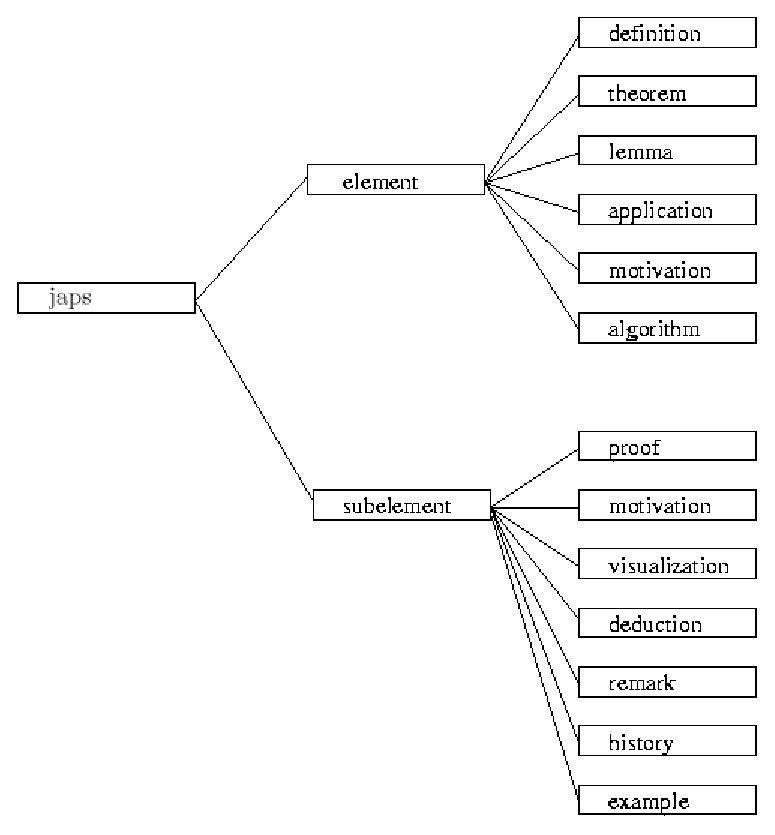
\includegraphics{pics/document_types.eps}
\end{center}
\caption{Dokumentklassen-Hierarchie}
\end{figure}

Entsprechend lauten die \cmdname{documentclass}-Deklarationen wie folgt:

\begin{verbatim}
\documentclass{japs.element.definition}
\documentclass{japs.element.theorem}
...
...
\documentclass{japs.subelement.remark}
\documentclass{japs.subelement.history}
\end{verbatim}

\remark{Vor dem endg"ultigen Release von Mumie 2 wird der Prefix "`japs"'
  wahrscheinlich noch in "`mumie"' ge"andert.}

\newpage

\section{Metainformationen}

Dabei handelt es sich um Informationen zum Dokument wie Name, Beschreibung,
Verfasser, verwendete Multimedia-Komponenten usw., die vom Autor des
Dokumentes spezifiziert werden m"ussen.

\subsection{Beispiel}\label{subsection:meta-example}

\begin{verbatim}
\documentclass{japs.element.definition}

 \begin{metainfo}
   \name{Lineare Unabh"angigkeit}
   \begin{description}
     Lineare Unabh"angigkeit, definiert "uber Nicht-Existenz einer
     nicht-trivialen Liniarkombination
   \end{description}
   \copyrightinfo{(c) 2007 Technische Universitaet Berlin}
   \status{pre}
   \begin{changelog}
     01.06.2007: Angefangen, noch unvollstaendig
     03.06.2007: Erster Entwurf
   \end{changelog}
   \begin{components}
     \component{image}{samples/images/img_vector.meta.xml}{bild_vektor}
     \component{applet}{samples/applets/LinearIndepemdence.meta.xml}{}
   \end{components}
   \begin{authors}
     \author{org/users/usr_kmueller.meta.xml}
     \author{org/users/usr_rmeier.meta.xml}
   \end{authors} \end{metainfo}

 \begin{content}
    ...
 \end{content}
\end{verbatim}

\subsection{Die \texttt{metainfo}-Umgebung}
Die Metainformationen folgen auf die Angabe der Dokumentenklasse wie folgt:

 \begin{verbatim}
 \begin{metainfo}
    ...
 \end{metainfo}\end{verbatim}

\subsection{Name}\label{name}

 \verb|\name{...}| - Name des Dokuments
 
 Erscheint z.B. in den Tooltips des Navigationsnetzes. Sollte nicht l"anger als
 etwa 80 Zeichen sein. Zu lange Worte vermeiden, da diese evtl.\ nicht in das
 Tooltip-Fenster passen! Bei Definitionen und Theoremen sollte der Name dem
 kausalen Begriff entsprechen, wie er auch im \verb|\title|- oder
 \verb|\defnotion|-Kommando angegeben wird (s. Kap. \ref{defnotion}). Einen
 Hinweis auf die Kategorie (Definition, Theorem, \dots) sollte der Name nicht
 enthalten, da die Kategorie ohnehin als Metainformation automatisch
 gespeichert wird. Also nicht "`Definition der Stetigkeit"', sondern einfach
 "`Stetigkeit"'.

 Der Name ist "`Plain Text"'. Umlaute sind aber erlaubt. Falls mathematische
 Formeln unumg"anglich sind, diese in \MmTeX-Code angeben. Beispiel:
 \verb'$\R^n$'.

 \remark{In zuk"unftigen Mumie-Versionen ist geplant, diese eingebetteten
   \MmTeX-Formeln dort, wo es m"oglich ist, in MathML zu "ubersetzen, so dass
   sie normal am Bildschirm angezeigt werden k"onnen.}

\subsection{Beschreibung (Description)}

 \begin{verbatim}
   \begin{description}
      ...
   \end{description} \end{verbatim}
 
 Kurze Beschreibung des Dokuments

 Kann ebenfalls in den Tooltips des Navigationsnetzes erscheinen. Sollte nicht
 l"anger als vier Zeilen a 80 Zeichen sein. Zu lange Worte vermeiden, da diese
 evtl.\ nicht in das Tooltip-Fenster passen!

 Die Beschreibung ist "`Plain Text"'. Umlaute sind aber erlaubt. Falls mathematische
 Formeln unumg"anglich sind, diese in \MmTeX-Code angeben. Beispiel:
 \verb'$\R^n$'. (Siehe auch Bemerkung oben).

\subsection{Copyright}

  \begin{verbatim}  \copyrightinfo{...}   \end{verbatim}

Enth�lt die Copyrightangaben.

\subsection{Autoren (Authors)}

\begin{verbatim}\begin{authors}
  \author{org/users/usr_kmueller.meta.xml}
  \author{org/users/usr_rmeier.meta.xml}
\end{authors}\end{verbatim}

Die Autoren des Dokuments

Jeder \verb'\author'-Befehl spezifiziert einen Autor. Das Argument ist der Pfad
zur Master-Datei des Autors als Benutzer des Systems.


\subsection{Komponenten}\label{subsection: Komponenten}

\begin{verbatim}\begin{components}
  \component{image}{samples/images/img_vector.meta.xml}{bild_vektor}
  \component{applet}{samples/applets/LinearIndepemdence.meta.xml}{}
\end{components}\end{verbatim}

Die verwendeten Komponenten

Jeder \verb'\component'-Befehl spezifiziert eine Komponente. Das erste Argument
ist der Typ der Komponente, das zweite der Pfad zur Master-Datei der
Komponente, das dritte die sognannte \emph{Binnen-Id}, auch lokale Id genannt.
Die Binnen-Id ist ein lokaler Bezeichner, mit dem die Komponente innerhalb des
Dokuments referenziert wird. Sie darf normale Buchstaben (keine Umlaute o."a),
Zahlen und die Zeichen \verb'_-.' enthalten.

\subsection{Status}\label{subsection: status}

  \begin{verbatim}  \status{...}   \end{verbatim}

Der Status des Dokuments. Das Argument des \verb'\status'-Befehls muss eines
der folgenden Schl"usselworte sein:

\begin{itemize}
\item \texttt{pre} -- in der Entwicklung
\item \texttt{devel\_ok} -- fertig aber ungepr\"uft
\item \texttt{content\_ok} -- inhaltlich nicht komplett aber brauchbar, technisch ungepr\"uft
\item \texttt{content\_complete} -- inhaltlich komplett, technisch ungepr\"uft
\item \texttt{ok\_for\_publication} -- inhaltlich nicht komplett aber brauchbar, technisch ok
\item \texttt{final} -- inhaltlich komplett, technisch ok
\end{itemize}

\remark{Diese Metainformation wird momentan nicht ausgewertet. Sie wird in
  Zukunft ge"andert oder ganz entfallen. Momentan muss sie aber noch angegeben werden.}


\subsection{Die \texttt{changelog}-Umgebung}\label{subsection: changelog}

Aus den Eintragungen der \texttt{changelog}--Umgebung wird die Metainformation
\textsl{Changelog} erzeugt. Sie soll die Kommunikation zwischen den beteiligten Personen
unterst\"utzen und Bemerkungen zum Inhalt des Dokuments enthalten. Dies k\"onnen auch
technische Details sein.  Zu beachten bleibt, dass allgemeinere technische Probleme (z.B.
fehlende MmTeX-Komandos), deren L\"osung eine Mitarbeit der Entwickler erfordert, weiterhin
\"uber das Bugreport-System kommuniziert werden. In der \texttt{changelog}--Umgebung kann
jeder Autor seine \"Anderungen und Pr\"ufberichte - insbesondere nach nicht bestandenem
Check - protokollieren. Konvention ist, dass das \textsl{Changelog} nie gel\"oscht, sondern
immer nur erg\"anzt wird. Die \texttt{changelog}--Umgebung hat folgende Gestalt:

\begin{verbatim}
\begin{changelog}
...
\end{changelog}
\end{verbatim}

\newpage

\section{Templates}\label{section:templates}

Die einzelnen Dokumenttypen (s. Kap. \ref{section:doctypes}) k\"onnen unterschiedliche
Strukturen aufweisen (s. Style-Guide \glqq How to write\grqq). F\"ur jede erlaubte Struktur
wird dem Autor ein \texttt{mumie}\TeX-Template zur Verf\"ugung gestellt, um die Eingabe zu
erleichtern.

Die Verwendung der Freestyle-Umgebung wird bei der Festlegung der Dokumentenklasse als
Parameter ``[freeenv]'' angegeben. Die anderen Styles ergeben sich aus den
\texttt{mumie}\TeX-Befehlen im Dokument und m\"ussen nicht gesondert angegeben werden.

\subsection{Templates zur Dokumentklasse \texttt{japs.element.definition}}

Alle Definitionen (bis auf Freestyle) k\"onnen optional Bemerkungen enthalten. Dazu siehe:
\ref{subsubsection:simpledef}.

\label{defnotion} Alle Definitionen enthalten statt dem \verb|\title{}|-Kommando das
Kommando \verb|\defnotion{}|, in dem der zu definierende kanonische Begriff unflektiert in
TeX-Schreibweise angegeben wird (z.B. \verb|\defnotion{linear abh"angig}| oder
\verb|\defnotion{Vektorraum $\R^n$|). Bei Mehrfachdefinitionen werden die Begriffe durch
Kommas getrennt (z.B. \verb|\defnotion{injektiv, surjektiv, bijektiv}|). Unter Bemerkungen
erg\"anzte Begriffe geh\"oren nicht in diese Aufz\"ahlung.

Das \verb|\title{}|-Kommando ist nicht zul\"assig. Unflektiert bedeutet u.a. in der Einzahl
(Ausnahme z.B. \verb|\defnotion{Multiplikation von Matrizen}|) und auch mit korrekter
Gro\"s-/Kleinschreibung (z.B. adjungierte Matrix). Die Eintr\"age unter
\verb|\defnotion{...}| sollen unter Einschr\"ankungen (s. Kap. \ref{name}) mit denen in
\verb|\name{...}| \"ubereinstimmen. Gro\"s- und Kleinschreibung sollen hier allerdings
orthografisch einer \"Uberschrift entsprechen, z.B. Lineare Unabh\"angigkeit.

\subsubsection{Freestyle}

\begin{figure}[h]
\centering
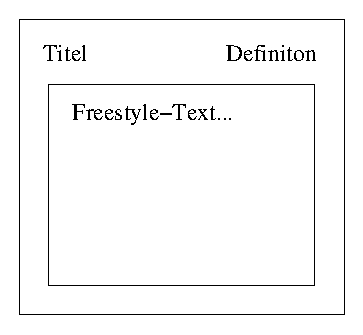
\includegraphics{pics/definition_freestyle.eps}
\caption{Layout Freestyle-Definition}
\end{figure}



\begin{verbatim}

\documentclass[freeenv]{japs.element.definition}

\begin{metainfo}\end{verbatim} [siehe Beispiel
\ref{subsection:meta-example}]\begin{verbatim}\end{metainfo}

\begin{content}
  \defnotion{.., ..,  ...  .., ..}
  ...
\end{content}
\end{verbatim}

\newpage

\subsubsection{Side-By-Side}

\begin{figure}[h]
\centering
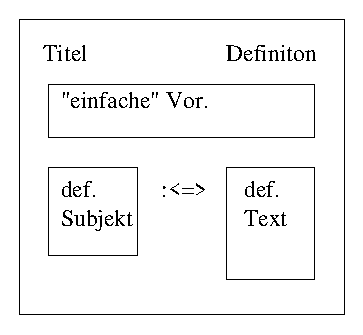
\includegraphics{pics/definition_side-by-side.eps}
\caption{Layout Side-By-Side-Definition}
\end{figure}


\begin{verbatim}
\documentclass{japs.element.definition}

\begin{metainfo}\end{verbatim}   [siehe Beispiel \ref{subsection:meta-example}]\begin{verbatim}\end{metainfo}

\begin{content}

 \defnotion{.., ..,  ...  .., ..}

 \begin{suppositions}
  ...
 \end{suppositions}

 \begin{defequivalence}[side-by-side]
    ...
   \isdefinedas
    ...
 \end{defequivalence}


\end{content}
\end{verbatim}

\newpage

\subsubsection{Top-Bottom}

\begin{figure}[h]
\centering
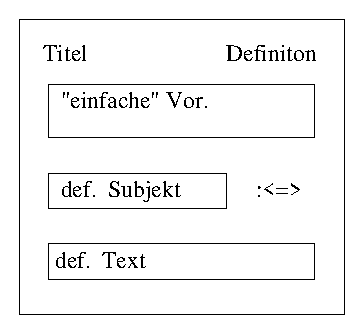
\includegraphics{pics/definition_top-bottom.eps}
\caption{Layout Top-Bottom-Definition}
\end{figure}


\begin{verbatim}
\documentclass{japs.element.definition}

\begin{metainfo}\end{verbatim}   [siehe Beispiel \ref{subsection:meta-example}]\begin{verbatim}\end{metainfo}

\begin{content}

 \defnotion{.., ..,  ...  .., ..}

 \begin{suppositions}
  ...
 \end{suppositions}

 \begin{defequivalence}[top-bottom]
    ...
   \isdefinedas
    ...
 \end{defequivalence}


\end{content}
\end{verbatim}
\newpage


\subsubsection{Mehrfach-Definition}\label{section:multipledef}

Zus\"atzlich zu den drei Definitionstypen sind \glqq Mehrfach\grqq-Defintionen m\"oglich, die die
folgende Form haben k\"onnen:

\begin{figure}[h]
\centering
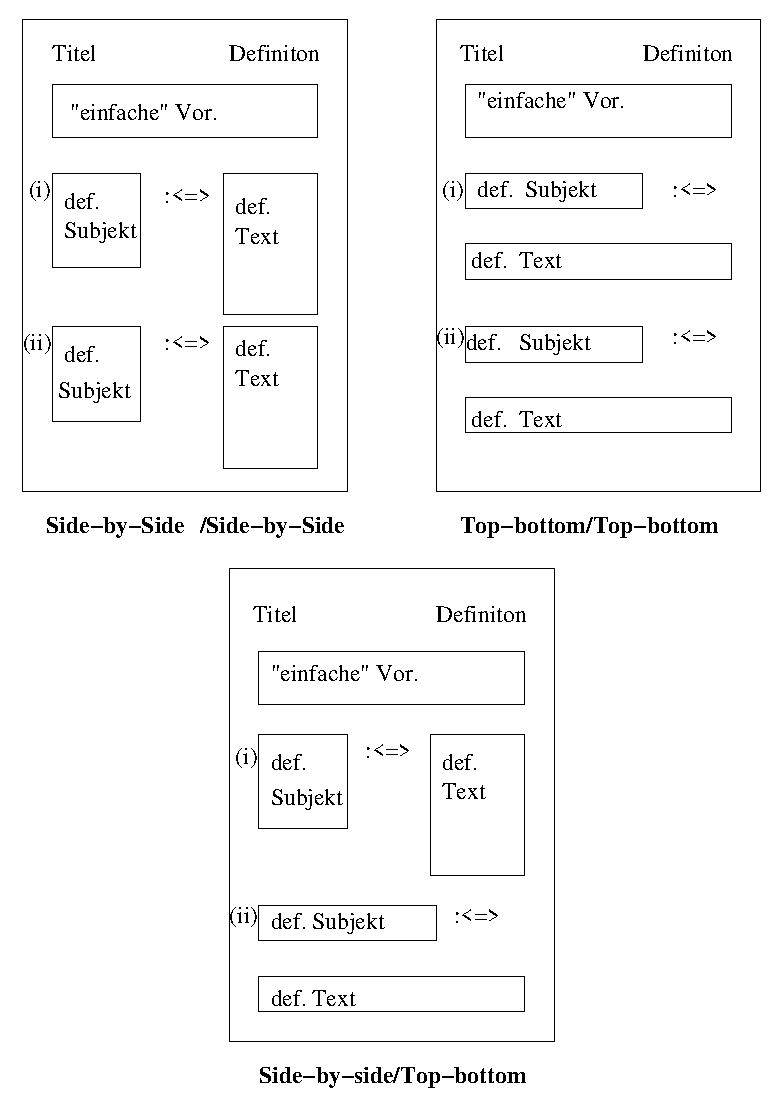
\includegraphics{pics/multiple_definition.eps}
\caption{Verschiedene M\"oglichkeiten der Mehrfachdefinition}
\end{figure}

Die \verb+defequivalence+-Umgebung kann dabei in beliebiger Anzahl jeweils mit
beliebigem optionalem Argument (\verb+side-by-side+, \verb+top-bottom+) auftauchen.
(s.u.)
\newpage

\begin{verbatim}

\documentclass{japs.element.definition}

\begin{metainfo}\end{verbatim}   [siehe Beispiel \ref{subsection:meta-example}]\begin{verbatim}\end{metainfo}

\begin{content}

 \defnotion{.., ..,  ...  .., ..}

 \begin{suppositions}
  ...
 \end{suppositions}

 \begin{defequivalence}[top-bottom]
    ...
   \isdefinedas
    ...
 \end{defequivalence}

 \begin{defequivalence}[side-by-side]
    ...
   \isdefinedas
    ...
 \end{defequivalence}


\end{content}
\end{verbatim}

\newpage

\subsubsection{Einfache Definition}\label{subsubsection:simpledef}

\begin{figure}[h]
\centering
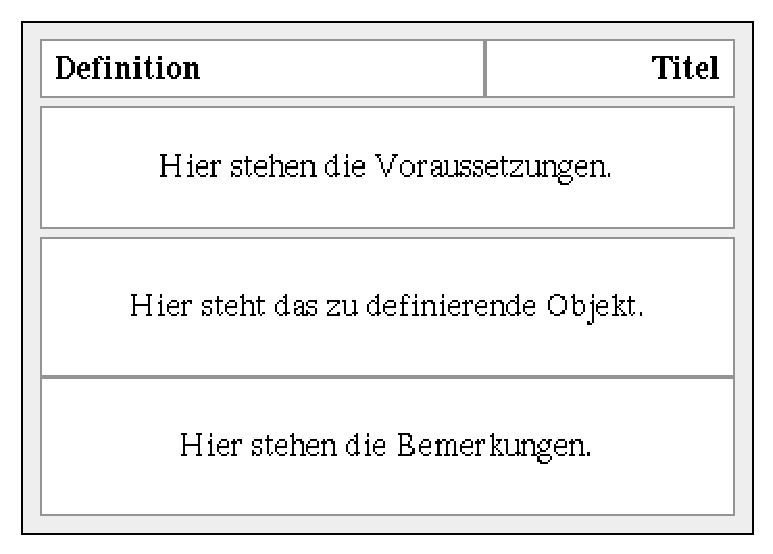
\includegraphics{pics/definition_simple.eps}
\caption{Layout Einfache Definition}
\end{figure}


\begin{verbatim}
\documentclass{japs.element.definition}

\begin{metainfo}\end{verbatim}   [siehe Beispiel \ref{subsection:meta-example}]\begin{verbatim}\end{metainfo}

\begin{content}

 \defnotion{.., ..,  ...  .., ..}

 \begin{suppositions}
  ...
 \end{suppositions}

 \begin{statement}
  ...
 \end{statement}

 \begin{remarks}
  ...
 \end{remarks}

\end{content}
\end{verbatim}


\newpage
\subsection{Templates zur Dokumentklasse \texttt{japs.element.theorem}}
\label{section:templatestheorem}

F\"ur das \verb|\title|-Kommando der Theoreme gelten die gleichen Aussagen, wie f\"ur das
\verb|\defnotion|-Kommando der Definitionen (s. Kap. \ref{defnotion}). Alle Theoreme
k\"onnen optional Bemerkungen enthalten. Dazu siehe: \ref{subsubsection:simpletheorem}.

\subsubsection{Freestyle}

\begin{figure}[h]
\centering
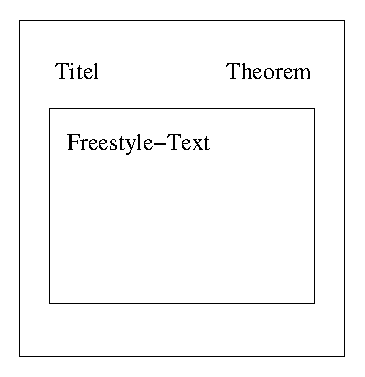
\includegraphics{pics/theorem_freestyle.eps}
\caption{Layout Freestyle-Theorem}
\end{figure}

\begin{verbatim}

\documentclass[freeenv]{japs.element.theorem}

\begin{metainfo}\end{verbatim}   [siehe Beispiel \ref{subsection:meta-example}]\begin{verbatim}\end{metainfo}

\begin{content}
  \title{...}
  ...
\end{content}
\end{verbatim}
\newpage

\subsubsection{Implikation: Side-By-Side}


\begin{figure}[h]
\centering
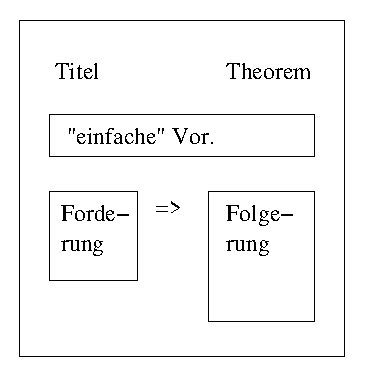
\includegraphics{pics/theorem_implication_side-by-side.eps}
\caption{Layout Side-By-Side-Theorem}
\end{figure}


\begin{verbatim}
\documentclass{japs.element.theorem}

\begin{metainfo}\end{verbatim}   [siehe Beispiel \ref{subsection:meta-example}]\begin{verbatim}\end{metainfo}

\begin{content}

 \title{...}

 \begin{suppositions}
  ...
 \end{suppositions}

 \begin{implication}[side-by-side]
    ...
   \implies
    ...
 \end{implication}


\end{content}
\end{verbatim}

\newpage

\subsubsection{Implikation: Top-Bottom}

\begin{figure}[h]
\centering
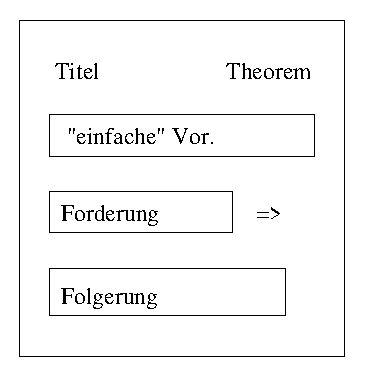
\includegraphics{pics/theorem_implication_top-bottom.eps}
\caption{Layout Top-Bottom-Theorem, Implikation}
\end{figure}


\begin{verbatim}
\documentclass{japs.element.theorem}

\begin{metainfo}\end{verbatim}   [siehe Beispiel \ref{subsection:meta-example}]\begin{verbatim}\end{metainfo}

\begin{content}

 \title{...}

 \begin{suppositions}
  ...
 \end{suppositions}

 \begin{implication}[top-bottom]
    ...
   \implies
    ...
 \end{implication}


\end{content}
\end{verbatim}

\newpage

\subsubsection{\"Aquivalenz: Side-By-Side}


\begin{figure}[h]
\centering
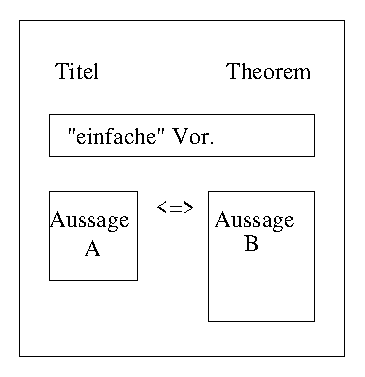
\includegraphics{pics/theorem_equivalence_side-by-side.eps}
\caption{Layout Side-By-Side-Theorem, \"Aquivalenz}
\end{figure}


\begin{verbatim}
\documentclass{japs.element.theorem}

\begin{metainfo}\end{verbatim}   [siehe Beispiel \ref{subsection:meta-example}]\begin{verbatim}\end{metainfo}

\begin{content}

 \title{...}

 \begin{suppositions}
  ...
 \end{suppositions}

 \begin{equivalence}[side-by-side]
    ...
   \isequivalentto
    ...
 \end{equivalence}


\end{content}
\end{verbatim}

\newpage

\subsubsection{\"Aquivalenz: Top-Bottom}

\begin{figure}[h]
\centering
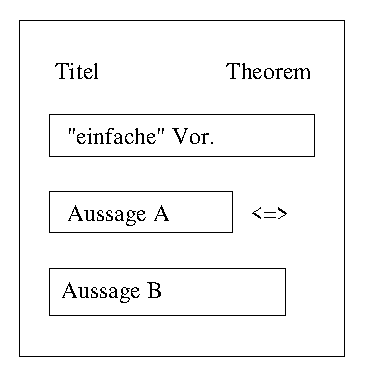
\includegraphics{pics/theorem_equivalence_top-bottom.eps}
\caption{Layout Top-Bottom-Theorem, \"Aquivalenz}
\end{figure}

\begin{verbatim}
\documentclass{japs.element.theorem}

\begin{metainfo}\end{verbatim}   [siehe Beispiel \ref{subsection:meta-example}]\begin{verbatim}\end{metainfo}

\begin{content}

 \title{...}

 \begin{suppositions}
  ...
 \end{suppositions}

 \begin{equivalence}[top-bottom]
    ...
   \isequivalentto
    ...
 \end{equivalence}

\end{content}
\end{verbatim}

\newpage

\subsubsection{Mehrfachtheoreme}

Hier gelten die gleichen Regeln wie bei den Mehrfachdefinitionen (s. Abschnitt
\ref{section:multipledef}), d.h.
die Umgebungen \verb+equivalence+ und \verb+implication+ k\"onnen (auch untereinander
kombiniert) beliebig oft mit jeweils belibigem optionalem Argument (\verb+side-by-side+,
\verb+top-bottom+) hintereinander auftauchen.

\subsubsection{Liste von Aussagen}

\begin{figure}[h]
\centering
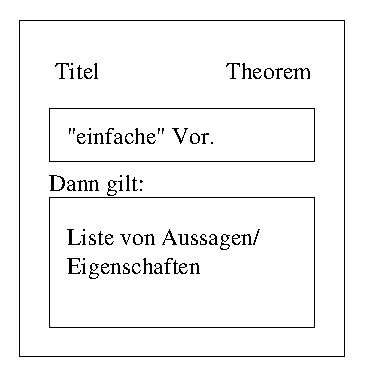
\includegraphics{pics/theorem_property-list.eps}
\caption{Layout Liste von Eigenschaften/Aussagen}
\end{figure}


\begin{verbatim}
\documentclass{japs.element.theorem}

\begin{metainfo}\end{verbatim}   [siehe Beispiel \ref{subsection:meta-example}]\begin{verbatim}\end{metainfo}

\begin{content}

 \title{...}

 \begin{suppositions}
  ...
 \end{suppositions}

\begin{propositionlist}
 \proposition ...
 \proposition ...
 \proposition ...
 ...
\end{propositionlist}

\end{content}
\end{verbatim}



\newpage

\subsubsection{Liste von \"aquivalenten Aussagen}

\begin{figure}[h]
\centering
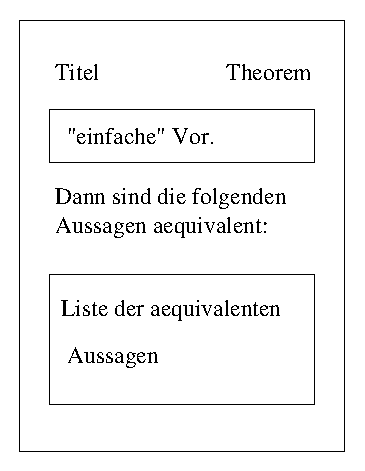
\includegraphics{pics/theorem_property-list_equivalent.eps}
\caption{Layout Liste von \"aquivalenten Eigenschaften/Aussagen}
\end{figure}


\begin{verbatim}
\documentclass{japs.element.theorem}

\begin{metainfo}\end{verbatim}   [siehe Beispiel \ref{subsection:meta-example}]\begin{verbatim}\end{metainfo}

\begin{content}

 \title{...}

 \begin{suppositions}
  ...
 \end{suppositions}

\begin{propositionlist}[equivalent]
\proposition ...
\proposition ...
\proposition ...
...
\end{propositionlist}

\end{content}
\end{verbatim}

\newpage

\subsubsection{Einfaches Theorem}\label{subsubsection:simpletheorem}.

\begin{figure}[h]
\centering
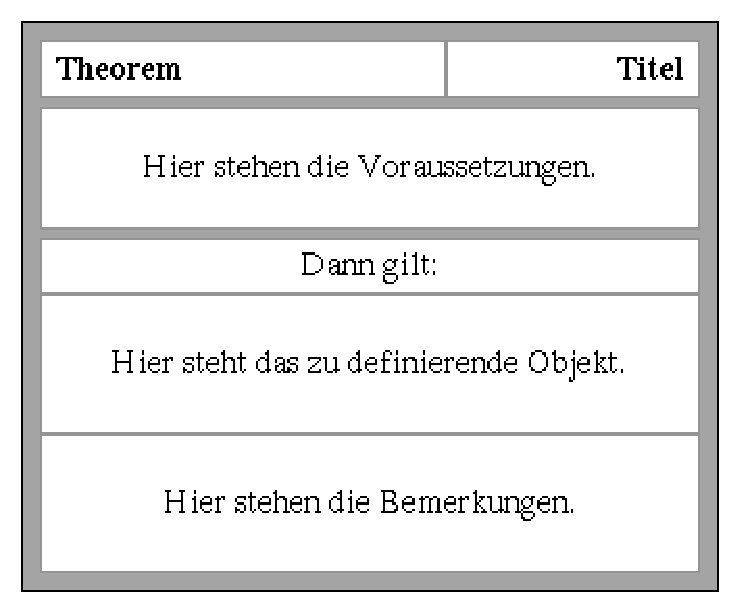
\includegraphics{pics/theorem_simple.eps}
\caption{Layout Einfaches Theorem}
\end{figure}

\begin{verbatim}
\documentclass{japs.element.theorem}

\begin{metainfo}\end{verbatim}   [siehe Beispiel \ref{subsection:meta-example}]\begin{verbatim}\end{metainfo}

\begin{content}

 \title{...}

 \begin{suppositions}
  ...
 \end{suppositions}

 \begin{statement}
  ...
 \end{statement}

 \begin{remarks}
  ...
 \end{remarks}

\end{content}
\end{verbatim}

\subsection{Templates zur Dokumentklasse \texttt{japs.element.lemma}}

Wie im Style-Guide \glqq How to write\grqq\/ angegeben, gibt es f\"ur
die Dokumentklasse \verb+lemma+ die gleichen M\"oglichkeiten bei der
Dokumentklasse \verb+theorem+ (siehe also Kap.
\ref{section:templatestheorem}). Damit sind f�r \verb+lemma+
die gleichen Umgebungen definiert wie f�r \verb+theorem+.

\newpage

\subsection{Templates f\"ur die Dokumentklasse \texttt{japs.element.algorithm}}

\subsubsection{Side-By-Side}

\begin{figure}[h]
\centering
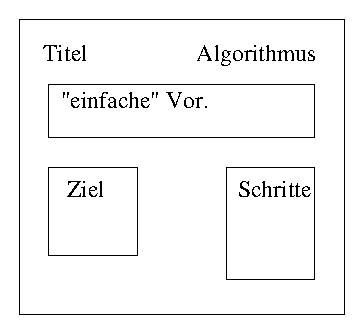
\includegraphics{pics/algorithm_side-by-side.eps}
\caption{Layout Algorithmus Side-By-Side}
\end{figure}

Die \verb|background|-Umgebung ist optional und soll die M�glichkeit bieten, die tragenden Ideen eines Algorithmus in knapper Form zu pr�sentieren.

\begin{verbatim}
\documentclass{japs.element.algorithm}

\begin{metainfo}\end{verbatim}   [siehe Beispiel \ref{subsection:meta-example}]\begin{verbatim}\end{metainfo}

\begin{content}

 \title{...}

 \begin{input}
  ...
 \end{input}

 \begin{output}
  ...
 \end{output}
 
 \begin{background}
  ...
 \end{background}

 \begin{algsteps}[side-by-side]
  \algstep ...
  \algstep ...
  ...
 \end{algsteps}

\end{content}
\end{verbatim}

\newpage

\subsubsection{Top-Bottom}

\begin{figure}[h]
\centering
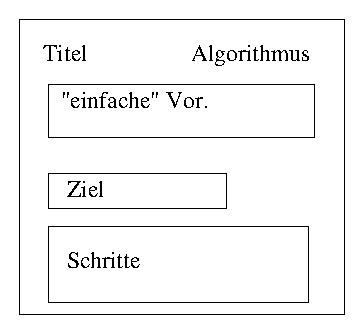
\includegraphics{pics/algorithm_top-bottom.eps}
\caption{Layout Algorithmus Top-Bottom}
\end{figure}


\begin{verbatim}
\documentclass{japs.element.algorithm}

\begin{metainfo}\end{verbatim}   [siehe Beispiel \ref{subsection:meta-example}]\begin{verbatim}\end{metainfo}

\begin{content}

 \title{...}

 \begin{input}
  ...
 \end{input}

 \begin{output}
  ...
 \end{output}
 
 \begin{background}
  ...
\end{background}

 \begin{algsteps}[top-bottom]
  \algstep ...
  \algstep ...
  ...
 \end{algsteps}
\end{content}
\end{verbatim}

\newpage


\subsection{Template f\"ur die Dokumentklasse \texttt{japs.element.motivation}}
\label{section:motivationtemplate}

F\"ur das Element \glqq Motivation\grqq\/ existiert kein festes Layout, sondern nur eine
Freestyle-Version.


\begin{figure}[h]
\centering
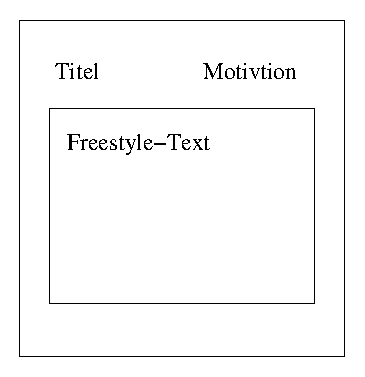
\includegraphics{pics/motivation_element.eps}
\caption{Layout Motivation (Element)}
\end{figure}

\begin{verbatim}
\documentclass[freeenv]{japs.element.motivation}

\begin{metainfo}\end{verbatim}   [siehe Beispiel \ref{subsection:meta-example}]\begin{verbatim}\end{metainfo}

\begin{content}

 \title{...}


\end{content}
\end{verbatim}

\newpage


\subsection{Template f\"ur die Dokumentklasse \texttt{japs.element.application}}

F\"ur das Element \glqq Motivation\grqq\/ existiert kein festes Layout, sondern nur eine
Freestyle-Version, laut Styleguide \glqq How to write\grqq\/ wird jedoch ein bildhafter
Aufbau angestrebt.


\begin{figure}[h]
\centering
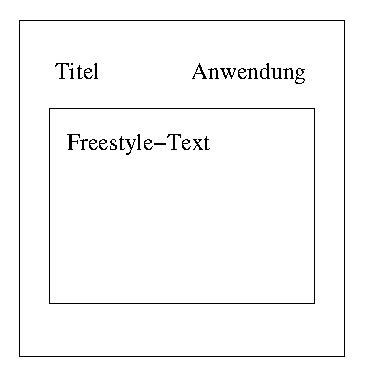
\includegraphics{pics/application.eps}
\caption{Layout Anwendung }
\end{figure}

\begin{verbatim}
\documentclass[freeenv]{japs.element.application}

\begin{metainfo}\end{verbatim}   [siehe Beispiel \ref{subsection:meta-example}]\begin{verbatim}\end{metainfo}

\begin{content}

 \title{...}


\end{content}
\end{verbatim}

\newpage

\subsection{Template f\"ur die Dokumentklasse \texttt{japs.subelement.proof}}

\begin{figure}[h]
\centering
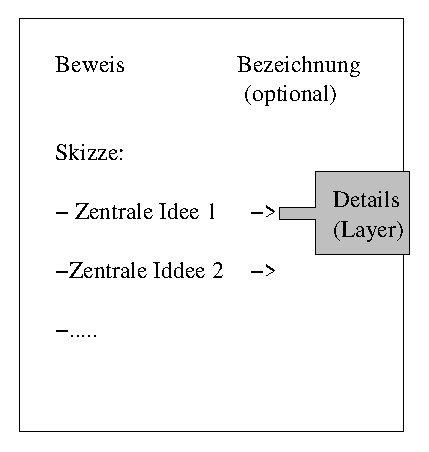
\includegraphics{pics/proof.eps}
\caption{Layout Beweis}
\end{figure}

\begin{verbatim}
\documentclass{japs.subelement.proof}

\begin{metainfo}\end{verbatim}   [siehe Beispiel \ref{subsection:meta-example}]\begin{verbatim}\end{metainfo}

\begin{content}

 \title{...}

 \begin{suppositions}
  ...
 \end{suppositions}

 \begin{steps}
  \step {Zentrale Idee1} Details...
  \step {Zentrale Idee2} Details...
  ...
 \end{steps}

\end{content}
\end{verbatim}


\subsection{Template f\"ur die Dokumentklasse \texttt{japs.subelement.deduction}}

\begin{figure}[h]
\centering
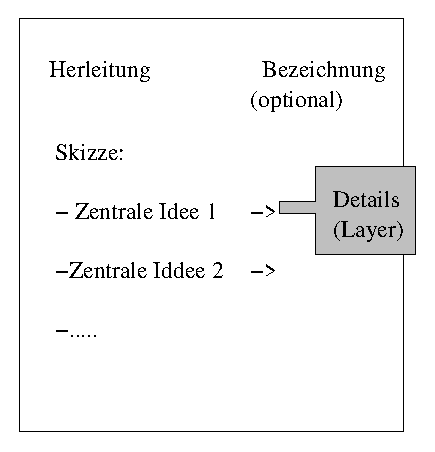
\includegraphics{pics/deduction.eps}
\caption{Layout Beweis}
\end{figure}

\begin{verbatim}
\documentclass{japs.subelement.deduction}

\begin{metainfo}\end{verbatim}   [siehe Beispiel \ref{subsection:meta-example}]\begin{verbatim}\end{metainfo}

\begin{content}

 \title{...}

 \begin{suppositions}
  ...
 \end{suppositions}

 \begin{steps}
  \step {zentrale Idee1} Details...
  \step {zentrale Idee2} Details...
  ...
 \end{steps}

\end{content}
\end{verbatim}


\subsection{Template f\"ur die Dokumentklasse \texttt{japs.subelement.motivation}}

Es gilt das gleiche wie f\"ur das Element \glqq Motivation\grqq\/, siehe hierzu Kap. \ref{section:motivationtemplate}.

\subsection{Templates f\"ur die Dokumentklasse \texttt{japs.subelement.history}}

Laut Styleguide \glqq How to write\grqq\/ und dem \texttt{mumieXML}-Styleguide
sind drei verschiedene Arten des Subelementes \glqq Historisches\grqq\/ vorgesehen,
eine mit personenbezogenen Informationen (biographisch), eine, die historische Informationen
zu einem mathematischen Gebiet oder Zweig enth\"alt und eine dritte, die einzelne,
bedeutende Ergebnisse betont.

\subsubsection{Biographisch}

\begin{figure}[h]
\centering
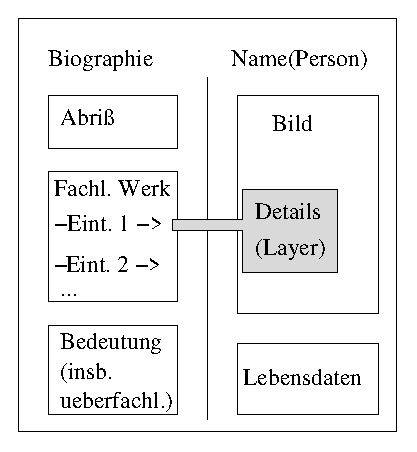
\includegraphics{pics/history_biographic.eps}
\caption{Layout Historisches (biographisch)}
\end{figure}

\begin{verbatim}
\documentclass{japs.subelement.history}

\begin{metainfo}\end{verbatim}   [siehe Beispiel \ref{subsection:meta-example}]\begin{verbatim}\end{metainfo}

\begin{content}

\begin{biography}
 \name{...}
 \picture{...}
 \lifespan["Todesdatum"]{"Geburtsdatum"}
\end{biography}

\begin{abstract}
 ...
\end{abstract}

\begin{mathactivity}
 \subject{...} ...
 \subject{...} ...
 ...
\end{mathactivity}

\begin{histrelevance}
 ...
\end{histrelevance}

\end{content}
\end{verbatim}


\subsubsection{Mathematisches Gebiet}

\begin{figure}[h]
\centering
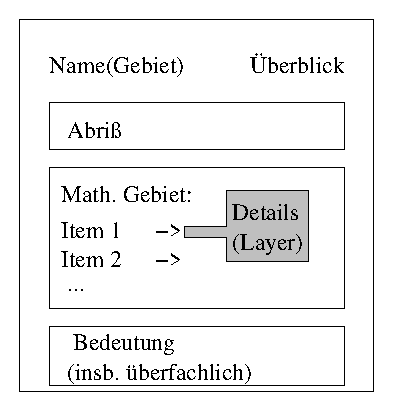
\includegraphics{pics/history_field.eps}
\caption{Layout Historisches (mathematisches Gebiet)}
\end{figure}


\begin{verbatim}
\documentclass{japs.subelement.history}

\begin{metainfo}\end{verbatim}   [siehe Beispiel \ref{subsection:meta-example}]\begin{verbatim}\end{metainfo}

\begin{content}

\title{...}

\begin{abstract}
 ...
\end{abstract}

\begin{mathactivity}
 \subject{...} ...
 \subject{...} ...
 ...
\end{mathactivity}

\begin{histrelevance}
 ...
\end{histrelevance}

\end{content}
\end{verbatim}



\subsubsection{Einzelnes Ergebnis}

\begin{figure}[h]  
\centering
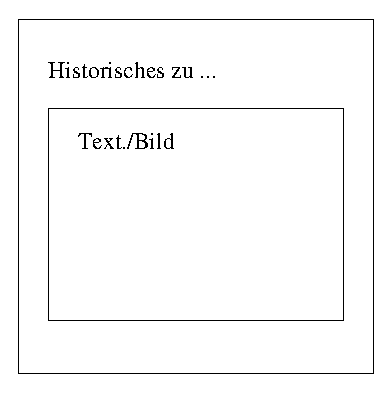
\includegraphics{pics/history_single-result.eps}
\caption{Layout Historisches (einzelnes Ergebnis)}
\end{figure}


\begin{verbatim}
\documentclass[freeenv]{japs.subelement.history}

\begin{metainfo}\end{verbatim}   [siehe Beispiel \ref{subsection:meta-example}]\begin{verbatim}\end{metainfo}

\begin{content}

 \title{...}

\end{content}
\end{verbatim}


\newpage


\subsection{Template f\"ur die Dokumentklasse \texttt{japs.subelement.remark}}

Laut \texttt{mumieXML}-Styleguide soll es f\"ur das Subelement \glqq Bemerkung\grqq\/ keine
Layout-Vorschriften geben. Allerdings gibt es Alternativen, die den Inhalt bzw. die Bedeutung der
Bemerkung betreffen:

\begin{itemize}
\item sloppy \quad ... nicht mathematische lockere Formulierung
\item alarm \quad ... Achtung! Wichtiger Hinweis
\item reflection \quad ... Hintergrund, "Philosophisches"
\item associative \quad ... Assoziation zu \"ahnlichen Strukturen ...
\end{itemize}

Diese Information mu{\ss} im mumie\TeX gegeben werden. Eine Idee f\"ur das sp\"atere Layout w\"are ein f\"ur
jede Variante typisches Icon, das bei Setzen des entsprechenden Attributs automatisch in die Seite
eingebunden wird.


\begin{verbatim}
\documentclass[sloppy|alarm|reflection|associative]{japs.subelement.remark}

\begin{metainfo}\end{verbatim}   [siehe Beispiel \ref{subsection:meta-example}]\begin{verbatim}\end{metainfo}

\begin{content}

 \title{...}

\end{content}
\end{verbatim}

\subsection{Template f\"ur die Dokumentklasse \texttt{japs.subelement.example}}

Hier gibt es keine Layout-Vorgaben.

\begin{verbatim}
\documentclass[freeenv]{japs.subelement.example}

\begin{metainfo}\end{verbatim}   [siehe Beispiel \ref{subsection:meta-example}]\begin{verbatim}\end{metainfo}

\begin{content}

 \title{...}

\end{content}
\end{verbatim}

\subsection{Template f\"ur die Dokumentklasse \texttt{japs.subelement.test}}

Hier gibt es keine Layout-Vorgaben.

\begin{verbatim}
\documentclass[freeenv]{japs.subelement.test}

\begin{metainfo}\end{verbatim}   [siehe Beispiel \ref{subsection:meta-example}]\begin{verbatim}\end{metainfo}

\begin{content}

 \title{...}

\end{content}
\end{verbatim}

\subsection{Template f\"ur die Dokumentklasse \texttt{japs.subelement.visualization}}

Hier gibt es keine Layout-Vorgaben.

\begin{verbatim}
\documentclass[freeenv]{japs.subelement.visualization}

\begin{metainfo}\end{verbatim}   [siehe Beispiel \ref{subsection:meta-example}]\begin{verbatim}\end{metainfo}

\begin{content}

 \title{...}

\end{content}
\end{verbatim}


\newpage
\section{Multimedia-Komponenten}\label{subsection: multim_komp}

\subsection{Bilder}

Bilder werden mit dem Befehl \verb'\image' eingebunden. Seine Syntax lautet:

\verb'   \image{'\var{binnen\_id}\verb'}'

wobei \var{binnen\_id} die Binnen-Id des Bildes ist (vgl.\ Abschnit \ref{subsection:
  Komponenten} ).

\subsection{Applets}

F"ur Applets stehen der \verb'\applet'-Befehl und die \verb'applet'-Umgebung zur
Verf"ugung. Die Syntax lautet:

\verb' \applet['\var{breite}\verb']['\var{hoehe}\verb']{'\var{binnen\_id}\verb'}'

bzw.\

\begin{flushleft}
\verb' \begin{applet}['\var{breite}\verb']['\var{hoehe}\verb']{'\var{binnen\_id}\verb'}'\\
\verb'   \param{'\var{name1}\verb'}{'\var{wert1}\verb'}'\\
\verb'   \param{'\var{name2}\verb'}{'\var{wert2}\verb'}'\\
\verb'   ...'\\
\verb' \end{applet}'
\end{flushleft}

Hierbei ist \var{binnen\_id} die Binnen-Id des Applets (vgl.\ Abschnit \ref{subsection:
  Komponenten} ). Optional kann die Breite und/oder H"ohe in Pixeln angegeben werden. Befehl
und Umgebung verhalten sich gleich bis auf die Tatsache, dass im Fall der
\verb'applet'-Umgebung dem Applet Parameter "ubergeben werden k"onnen. Dies geschieht mit
dem Befehl \verb'\param'. Dessen beide Argumente stellen Namen und Wert des Parameters dar.

\section{Textauszeichnung}

\subsection{Hervorhebungen}

Ein einheitlicher Befehl anstelle der sonst in \LaTeX\ m\"oglichen Befehle f\"ur einfache
Hervorhebung von Texten:

\begin{verbatim}
 \emph{...}
\end{verbatim}

\subsection{Fachbegriffe, Definitionsbegriffe}

Vgl. oben; nur hier im Speziellen f\"ur Fachvokabular:

\begin{verbatim}
 \notion{...}
\end{verbatim}

\subsection{Code-Stil}

Angelehnt an die \verb+verbatim+-Umgebung in \LaTeX\ und den \verb+\verb+-Befehl:

\begin{enumerate}
\item In Display-Anordnung f\"ur l\"angere \glqq Programm-Code-Texte\grqq:
\begin{verbatim}
 \begin{code}
  ...
 \end{code}
\end{verbatim}

\item In Inline-Anordnung:

\begin{verbatim}
 \code{...}
\end{verbatim}

\end{enumerate}

\subsection{Tastatur-Eingabe-Stil}

Vgl. oben; nur hier im Speziellen f\"ur Tastatur-Eingaben:

\begin{verbatim}
  \keyb{...}
\end{verbatim}

\section{Listen und Tabellen}


%%%%%%%%%%%%%%%%%%%%%%%%%%%%%%%%%%%%%%%%%%%%%%%%%%%%%%%%%%%
%%                         Listen                        %%
%%%%%%%%%%%%%%%%%%%%%%%%%%%%%%%%%%%%%%%%%%%%%%%%%%%%%%%%%%%

\subsection{Listen}

\subsubsection{Beispiel f�r eine einfache Liste}\label{subsubsection:list-example-plain}

%  \newitemizeclasses{foo,bar}

\begin{verbatim}
  ...
  \begin{itemize}[circle]
    \item Eins

      Neuer Absatz

    \item Zwei
    \item drei
  \end{itemize}
  ...
\end{verbatim}

\subsubsection{Beispiel f�r eine nummerierte Liste}\label{subsubsection:list-example-enum}

\begin{verbatim}
  ...
  \begin{enumerate}
    \item Eins
    \begin{enumerate}[alph]
       \item Eins A
       \item Eins B
    \end{enumerate}
    \item Zwei
    \item Drei
  \end{enumerate}
  ...
\end{verbatim}

\subsubsection{Einfache Listen}

Eine einfache Liste wird durch folgende Umgebung eingeschlossen:

\begin{verbatim}
  ...
  \begin{itemize}[SYMBOL]
    ...
  \end{itemize}
  ...
\end{verbatim}

\begin{description}
\item[\texttt{SYMBOL}] Spezifiziert optional, welches Symbol den einzelnen
Punkten der Liste vorangestellt werden soll. Folgende Symbole sind verf�gbar:
\end{description}

    \begin{center}
    \begin{tabular}[c]{|c|c|c|c|c|}
        \hline
        Symbol&Darstellung\\
        \hline
        \texttt{normal}& $\cdot$ \\
        \texttt{bullet}& $\bullet$ \\
        \texttt{circle}& $\circ$ \\
        \texttt{square}& $\diamond$ \\
        \hline
    \end{tabular}
    \end{center}

\subsubsection{Nummerierte Listen}

Eine nummerierte Liste wird durch folgende Umgebung eingeschlossen:

\begin{verbatim}
  ...
  \begin{enumerate}[STYLE]
    ...
  \end{enumerate}
  ...
\end{verbatim}

\begin{description}
\item[\texttt{STYLE}] Spezifiziert optional, in welchem Stil die Liste
nummeriert werden soll. Folgende M�glichkeiten stehen zur Verf�gung:
\end{description}

    \begin{center}
    \begin{tabular}[c]{|c|c|c|c|c|}
        \hline
        Style&Beschreibung&Darstellung (z.B.: Punkt 14)\\
        \hline
        \texttt{arabic}& arabische Zahlen & 14.\\
        \texttt{roman}& r�mische Zahlen (klein) & xiv.\\
        \texttt{Roman}& r�mische Zahlen (gro�) & XIV.\\
        \texttt{alph}& alphabetisch (Kleinbuchstaben) & n.\\
        \texttt{Alph}& alphabetisch (Gro�buchstaben) & N.\\
        \texttt{greek}& griechisch (Kleinbuchstaben) & $\xi$. \\
        \hline
    \end{tabular}
    \end{center}

\subsubsection{Listenelemente}

\begin{verbatim}
  ...
  \item Listenpunkt
  ...
\end{verbatim}

Leitet die einzelen Punkte einer Liste ein.

Sowohl einfache als auch nummerierte Listen k�nnen in jedem
Unterpunkt ihrerseits wiederum einfache und/oder nummerierte Listen
enthalten. (Dazu siehe: \ref{subsubsection:list-example-enum}.)

\subsubsection{Benutzerdefinierte Listenklassen}

\begin{verbatim}
  ...
  \newitemizeclasses{CLASS,CLASS}
  ...
\end{verbatim}

Definiert neue, benutzerspezifische Listenklassen.

\begin{description}
\item[\texttt{CLASS}] Spezifikation der neu zu definierenden
benutzerspezifischen Listenklasse.
\end{description}


%%%%%%%%%%%%%%%%%%%%%%%%%%%%%%%%%%%%%%%%%%%%%%%%%%%%%%%%%%%
%%                        Tabellen                       %%
%%%%%%%%%%%%%%%%%%%%%%%%%%%%%%%%%%%%%%%%%%%%%%%%%%%%%%%%%%%

\subsection{Tabellen}

\subsubsection{Beispiel}\label{subsubsection:table-example}

\begin{verbatim}
   ...
   \begin{table}
    \head
      Inhalte Kopf 11 & 12 & 13
    \body
      \rowspan{2} 11 & 12 & 13 \\
      22 & 23 \\
      31 & 32 & 33 \\
      41 & \colspan{2} 42 43 \\
      \colspan{2}
      \begin{table}
        a & b \\
        c & d
      \end{table} & 0
  \end{table}
   ...
\end{verbatim}

\subsubsection{Die Tabelle und die generelle Ausrichtung der Inhalte}\label{subsubsection:table-param}

\remark{Dieser Abschnitt muss noch an "Anderungen in MmTeX angepasst werden}

\subsubsection{Kopf, Hauptteil, Fu�}

Innerhalb der Tabellenumgebung stehen folgende Befehle zur Verf�gung:

\begin{verbatim}
  \head
    ...
  \body
    ...
  \foot
    ...
\end{verbatim}

Sie leiten die jeweiligen Abschnitte ein. F�r den Hauptteil k�nnen
zus�tzlich optional Parameter f�r die Ausrichtung der Zellinhalte
jeder Spalte angeben werden. Dazu siehe: \ref{subsubsection:table-param}.
F�r jeden Abschnitt der Tabelle sind mehrere Zeilen erlaubt.

\remark{Dieser Abschnitt muss noch an "Anderungen in MmTeX angepasst werden}

\subsubsection{Zeilen, Spalten, Zellen}

\begin{verbatim}
  ...
  Inhalte Zelle 1 & Inhalte Zelle 2 & Inhalte Zelle 3 \\
  ...
\end{verbatim}

Zellen werden voneinander durch das Zeichen \texttt{\&} abgetrennt.
Jede Zeile der Tabelle wird durch zweifachen Backslash abgeschlossen.

\subsubsection{Zellenverbindungen}

\begin{verbatim}
  ...
    ... & \rowspan{rows} Inhalte & ... \\
  ...
    ... & \colspan{cols} Inhalte & ... \\
  ...
\end{verbatim}

Verbindung zweier oder mehrerer benachbarter Zellen in Zeilen bzw. Spalten.
Die Parameter \texttt{rows} bzw. \texttt{cols} spezifizieren die Anzahl
der zu verbindenen Zeilen bzw. Spalten. Optional kann auch hier f�r jeden
Verbund eine eigene Klasse angegeben werden. Dazu siehe: \ref{subsubsection:table-param}.

Spezifiziert benutzerdefinierte Klassen f�r Tabellen. Die Definition erfolgt
ausserhalb des \texttt{content}-Blocks und wird, wie im Beispiel gezeigt,
bei der �ffnung einer Tabellenumgebung referenziert.

\section{Kommentare}
Es gibt wie bei \LaTeX\ zwei Arten von Kommentaren.
\begin{enumerate}
  \item Der Rest einer Zeile wird mit \verb+ % + auskommentiert.
  \item Mehrzeilige Kommentare werden mit der Umgebung

    \verb+ \begin{comment}+

      \hspace{1cm}\textit{Kommentar}

    \verb+ \end{comment}+

erzeugt.
\end{enumerate}
\newpage

\section{Mathematische Befehle}
Ma\"stab f\"ur die zu implementierende mathematische Befehle stellt die Excel-Tabelle \texttt{mumietex\_list.xls} dar. Diese Tabelle befindet sich im berliner CVS \texttt{[JAPS]\slash notes}.

\subsection{Vektoren}
\subsubsection{Einfache Vektoren}

Der Befehl f\"ur einfache Vektoren lautet
\begin{center}
\verb+\vec{+\textit{Vektorname}\verb+}+
\end{center}
\paragraph{Beispiel:} 
\begin{math}
\vec{a}
\end{math}
wird erzeugt durch \verb+\vec{a}+ 
\subsubsection{Zeilenvektoren} 
Der Befehl f\"ur den Zeilenvektor
\begin{math}
\begin{pmatrix}
         v_1 & v_2 & \ldots & v_n 
\end{pmatrix}
\end{math}
lautet
\begin{verbatim}
\vector[r]{$v_1$ \\ $v_2$ \\ ... \\ $v_n$}
\end{verbatim}
\subsubsection{Spaltenvektoren}
Der Befehl f\"ur den Spaltenvektor
\begin{math}
\begin{pmatrix}
         v_1 \\ v_2 \\ \vdots \\ v_n
         \end{pmatrix}
         \end{math}
         lautet
\begin{verbatim}
         \vector[c]{$v_1$ \\ $v_2$ \\ $\ldots$ \\ $v_n$}
\end{verbatim}
%DG:  vectorstyle{arrow}, usw muss ich noch mit Tilman klaeren

\subsection{Mathematische Umgebungen}
Welche Umgebungen sind notwendig? Welche sind \"{u}berfl\"{u}ssig?
\begin{verbatim}
%DE: n�tig
  $...$
%DE: n�tig
  \[...\]
%DE: n�tig
  \begin{align}
    ...
  \end{align}
%DE: n�tig
  \begin{cases}
    -1 & x<0,\\
    1  & x>0,\\
    0  & \text{sonst}.
  \end{cases}
%DE: nicht n�tig
  \begin{subarray}
    ...
  \end{subarray}
%DE: nicht n�tig
  \phantom{...}
\end{verbatim}
\subsection{Funktionen}
    \begin{center}
    \begin{tabular}[c]{|c|c|c|c|c|}
        \hline
        $\sin$      & \verb+\sin+   & &$\log$      & \verb+\log+\\
        $\cos$      & \verb+\cos+   & &$\lg$       & \verb+\lg+\\
        $\tan$      & \verb+\tan+   & &$\ln$       & \verb+\ln+\\
        $\cot$      & \verb+\cot+   & &$\exp$      & \verb+\exp+\\
        $\sec$      & \verb+\sec+   & &$\det$      & \verb+\det+\\
        $\csc$      & \verb+\csc+   & &$\max$      & \verb+\max+\\
        $\gcd$      & \verb+\gcd+   & &$\min$      & \verb+\min+\\
        $\arcsin$   & \verb+\arcsin+& &$\sup$      & \verb+\sup+\\
        $\arccos$   & \verb+\arccos+& &$\inf$      & \verb+\inf+\\
        $\arctan$   & \verb+\arctan+& &$\lim$      & \verb+\lim+\\
        $\sinh$     & \verb+\sinh+  & &$\limsup$   & \verb+\limsup+\\
        $\cosh$     & \verb+\cosh+  & &$\liminf$   & \verb+\liminf+\\
        $\tanh$     & \verb+\tanh+  & &$\varlimsup$& \verb+\varlimsup+\\
        $\coth$     & \verb+\coth+  & &$\varliminf$& \verb+\varliminf+\\
        $\dim$      & \verb+\dim+   & &$\ker$      & \verb+\ker+\\
        $\deg$      & \verb+\deg+   & &$\hom$      & \verb+\hom+\\
        $\arg$      & \verb+\arg+   & &            & \\
        \hline
    \end{tabular}
    \end{center}


\subsection{Logische Symbole, Pfeile, Relationszeichen und Klammern}

\subsubsection{logische Symbole und Pfeile}
    \begin{center}
    \begin{tabular}[c]{|c|c|c|c|c|}
        \hline
            $\neg$              & \verb+\neg+           & & $\to$               & \verb+\to+\\
            $\Rightarrow$       & \verb+\Rightarrow+, \verb+\To+    & & $\leftarrow$        & \verb+\leftarrow+\\
            $\Leftarrow$        & \verb+\Leftarrow+     & & $\nLeftrightarrow$  & \verb+\nLeftrightarrow+\\
            $\Leftrightarrow$   & \verb+\Leftrightarrow+& & $\hookrightarrow$   & \verb+\hookrightarrow+\\
            $\iff$              & \verb+\iff+           & & $\nLeftarrow$       & \verb+\nLeftarrow+ \\
            $\lor$              & \verb+\lor+           & & $\nRightarrow$      & \verb+\nRightarrow+\\
            $\land$             & \verb+\land+         & & $\mapsto$           & \verb+\mapsto+\\
            $\rightarrow$       & \verb+\rightarrow+    & &           & \\
        \hline
    \end{tabular}
    \end{center}

\subsubsection{Relationszeichen:}
    \begin{center}
    \begin{tabular}[c]{|c|c|c|c|c|}
        \hline
        $=$             & \verb+=+   & & $\equiv$        & \verb+\equiv+\\
        $<$             & \verb+<+   & & $\thicksim$     & \verb+\thicksim+\\
        $>$             & \verb+>+   & & $\simeq$        & \verb+\simeq+\\
        $\not<$         & \verb+not<+& & $\approx$       & \verb+\approx+\\
        $\not>$         & \verb+not>+& & $\cong$         & \verb+\cong+\\
        $\leq$          & \verb+\leq+& & $\neq$          & \verb+\neq+\\
        $\geq$          & \verb+\geq+& &                 & \\
        \hline
    \end{tabular}
    \end{center}

\subsubsection{Klammern}
    \begin{center}
    \begin{tabular}[c]{|c|c|c|c|c|}
        \hline
        $($      & \verb+(+   & & $\langle$       & \verb+\langle+\\
        $)$      & \verb+)+   & & $\rangle$       & \verb+\rangle+\\
        $[$      & \verb+]+   & & $\|$            & \verb+\|+\\
        $]$      & \verb+]+   & & $|$             & \verb+|+\\
        $\{$     & \verb+\{+  & & $\mid$          & \verb+\mid+\\
        $\}$     & \verb+\}+  & & $\backslash$    & \verb+\backslash+\\
        $/$      & \verb+/+   & & $\backslash$    & \verb+\backslash+\\
        \hline
    \end{tabular}
    \end{center}

\subsection{Quantoren, Mengenlehre}

   \subsubsection{Quantoren}
   Quantoren werden in der alten Notation verwendet, das hei{\ss}t
   \verb+\exists+, \verb+\nexists+  und \verb+\forall+ ergibt die Ausgabe:
   \begin{center}
       $\exists$, $\nexists$ und $\forall$
   \end{center}

\subsubsection{Mengenlehre:}
    \begin{center}
    \begin{tabular}[c]{|c|c|c|c|c|}
        \hline
            $\subset$   & \verb+\subset+  & & $\bigcap$   & \verb+\bigcap+\\
            $\supset$   & \verb+\supset+  & & $\cup$      & \verb+\cup+\\
            $\subseteq$ & \verb+\subseteq+& & $\bigcup$   & \verb+\bigcup+\\
            $\supseteq$ & \verb+\supseteq+& & $\nsubseteq$& \verb+\nsubseteq+\\
            $\in$       & \verb+\in+      & & $\nsupseteq$& \verb+\nsupseteq+\\
            $\notin$    & \verb+\notin+   & & $\subsetneq$& \verb+\subsetneq+\\
            $\ni$       & \verb+\ni+      & & $\supsetneq$& \verb+\supsetneq+\\
            $\cap$      & \verb+\cap+     & & $\setminus$ & \verb+\setminus+\\
        \hline
    \end{tabular}
    \end{center}

\subsection{Summe, Produkt, Integral}
    \begin{center}
    \begin{tabular}[c]{|c|c|c|c|c|}
        \hline
        $\sum$        & \verb+\sum+  & & $\iiiint$   & \verb+\iiiint+\\
        $\prod$       & \verb+\prod+ & & $\idotsint$ & \verb+\idotsint+\\
        $\int$        & \verb+\int+  & & $\oint$     & \verb+\oint+\\
        $\iint$       & \verb+\iint+ & & &\\
        $\iiint$      & \verb+\iiint+& & &\\
        \hline
    \end{tabular}
    \end{center}

\subsection{Operatoren}
    \begin{center}
    \begin{tabular}[c]{|c|c|c|c|c|}
        \hline
            $+$         & \verb+++         & & $\times$    & \verb+\times+\\
            $-$         & \verb+-+         & & $\div$      & \verb+\div+\\
            $\pm$       & \verb+\pm+       & & $\oplus$    & \verb+\oplus+\\
            $\mp$       & \verb+\mp+       & & $\ominus$   & \verb+\ominus+\\
            $\cdot$     & \verb+\cdot+     & & $\otimes$   & \verb+\otimes+\\
            $:$         & \verb+:+         & & $\odot$     & \verb+\odot+\\
            $\vee$      & \verb+\vee+      & & $\bigoplus$ & \verb+\bigoplus+\\
            $\wedge$    & \verb+\wedge+    & & $\bigotimes$& \verb+\bigotimes+\\
            $\bigvee$   & \verb+\bigvee+   & & $\bigodot$  & \verb+\bigodot+\\
            $\bigwedge$ & \verb+\bigwedge+ & & $\circ$     & \verb+\circ+\\
        \hline
    \end{tabular}
    \end{center}

\subsection{Formelspezifische Zeichen}
    \begin{minipage}{\linewidth}
    \begin{center}
    \begin{tabular}[c]{|c|c|}
        \hline
        Bruch:        & \verb+\frac{+\textit{Z\"ahler}\verb+}{+\textit{Nenner}\verb+}+ \\
%DE: brauchen wir den Kettenbruch wirklich als extra Kommando?
        Kettenbruch:  & \verb+\cfrac{+\textit{Z\"ahler}\verb+}{+\textit{Nenner}\verb+}+ \\
        $\binom{n}{k}$& \verb+\binom{n}{k}+\\
        $x^k$         & \verb+x^{k}+ \\
        $x_k$         & \verb+x_{k}+ \\
        $\sqrt[n]{x}$ & \verb+\sqrt[+\textit{Exponent}\verb+]{x}+ \\
        $\dot{x}$     & \verb+\dot{x}+ \\
        $\ddot{x}$    & \verb+\ddot{x}+ \\
        $\dddot{x}$   & \verb+\dddot{x}+ \\
        $\ddddot{x}$  & \verb+\ddddot{x}+ \\
        $x'$          & \verb+x'+ \\
        $x''$         & \verb+x''+ \\
        $x'''$        & \verb+x'''+ \\
        \hline
    \end{tabular}
    \end{center}
    \end{minipage}

\subsection{Markierungen}
    \begin{center}
    \begin{tabular}[c]{|c|c|c|c|c|}
        \hline
        $\hat{x}$         & \verb+\hat{x}+         & & $\check{x}$       & \verb+\check{x}+\\
        $\widehat{xyz}$   & \verb+\widehat{xyz}+   & & $\bar{x}$         & \verb+\bar{x}+\\
        $\breve{x}$       & \verb+\breve{x}+       & & $\overline{xyz}$  & \verb+\overline{xyz}+\\
        $\acute{x}$       & \verb+\acute{x}+       & & $\underline{xyz}$ & \verb+\underline{xyz}+\\
        $\grave{x}$       & \verb+\grave{x}+       & & $\overbrace{xyz}$ & \verb+\overbrace{xyz}+\\
        $\tilde{x}$       & \verb+\tilde{x}+       & & $\underbrace{xyz}$& \verb+\underbrace{xyz}+\\
        $\widetilde{xyz}$ & \verb+\widetilde{xyz}+ & & $\underbrace{xyz}$& \verb+\underbrace{xyz}+\\
        $\mathring{x}$    & \verb+\mathring{x}+    & & $\underbrace{xyz}$& \verb+\underbrace{xyz}+\\
        \hline
    \end{tabular}
    \end{center}

\subsection{Sonstige mathematische Symbole}
    \begin{center}
    \begin{tabular}[c]{|c|c|c|c|c|}
        \hline
        $\infty$      & \verb+\infty+     & & $*$           & \verb+*+\\
        $\partial$    & \verb+\partial+   & & $\ldots$      & \verb+\ldots+\\
        $\nabla$      & \verb+\nabla+     & & $\cdots$      & \verb+\cdots+\\
        $\triangle$   & \verb+\triangle+  & & $\vdots$      & \verb+\vdots+\\
        $\varnothing$ & \verb+\varnothing+& & $\ddots$      & \verb+\ddots+\\
        $\emptyset$   & \verb+\emptyset+  & & $\%$          & \verb+\%+\\
        $!$           & \verb+!+          & & $\#$          & \verb+\#+ \\
        $\$$          & \verb+\$+         & & $\&$          & \verb+\&+ \\
        $\_$          & \verb+\_+         & &               & \verb++ \\
        \hline
    \end{tabular}
    \end{center}

\subsection{Sonstige nicht-mathematische Symbole}
(Evtl. in ein eigenes Kapitel, zusammen mit internationalen Bezeichnungen usw.)
    \begin{center}
    \begin{tabular}[c]{|c|c|c|c|c|}
        \hline
        *           & \verb+*+          & & \ldots        & \verb+\ldots+\\
        \S          & \verb+\S+         & & \vdots        & \verb+\vdots+\\
        \$          & \verb+\$+         & & -             & \verb+-+\\
        \_          & \verb+\_+         & & --            & \verb+--+\\
        \%          & \verb+\%+         & & ---           & \verb+---+\\
        \#          & \verb+\#+         & &            & \verb++\\
        \&          & \verb+\&+         & &               & \verb++\\
        \^{}        & \verb+^+          & &             & \verb++ \\
        \~{}        & \verb+\~{}+       & &             & \verb++ \\
        \hline
    \end{tabular}
    \end{center}

\subsection{Sonstige mathematische Befehle}
\begin{tabular}{l}
  \verb+\text{...}+\\
  \verb+\overset{...}{...}+\\
  \verb+\underset{...}{...}+\\
  \verb+\pmod{...}+\\
  \verb+\bmod+\\
\end{tabular}

\paragraph{Beispiele:}
\begin{enumerate}
  \item $\overset{\text{def}}{=}$ wird erzeugt mit \verb+\overset{\text{def}}{=}+.
  \item $a \equiv b \pmod{m}$ wird erzeugt mit \verb+a \equiv b \pmod{m}+.
  \item $a \bmod b$ wird erzeugt mit \verb+a \bmod b+.
\end{enumerate}

\subsection{Zahlenmengen}
    Zahlenmengen sind mit einem optionalen Argument ausgestattet,
    welches die Dimension angibt.
    Folgende Befehle stehen zur Verf"ugung:
    \begin{center}
%DE: wie bei \vector
        \verb+\N[+\textit{dim}\verb+]+\\
        \verb+\Z[+\textit{dim}\verb+]+\\
        \verb+\Q[+\textit{dim}\verb+]+\\
        \verb+\R[+\textit{dim}\verb+]+\\
        \verb+\C[+\textit{dim}\verb+]+\\
    \end{center}
    \paragraph{Beispiel:} $\mathbb{R}^n$ wird erzeugt mit \verb+\R[n]+.

\subsection{griechische Buchstaben}
    \begin{center}
    \begin{tabular}[c]{|c|c|c|c|c|}
        \hline
        $\alpha$  & \verb+\alpha+  & & $\tau$    & \verb+\tau+\\
        $\beta$   & \verb+\beta+   & & $\upsilon$& \verb+\upsilon+\\
        $\gamma$  & \verb+\gamma+  & & $\phi$    & \verb+\phi+\\
        $\delta$  & \verb+\delta+  & & $\chi$    & \verb+\chi+\\
        $\epsilon$& \verb+\epsilon+& & $\psi$    & \verb+\psi+\\
        $\zeta$   & \verb+\zeta+   & & $\omega$  & \verb+\omega+\\
        $\eta$    & \verb+\eta+    & & $\Gamma$  & \verb+\Gamma+\\
        $\theta$  & \verb+\theta+  & & $\Delta$  & \verb+\Delta+\\
        $\iota$   & \verb+\iota+   & & $\Theta$  & \verb+\Theta+\\
        $\kappa$  & \verb+\kappa+  & & $\Lambda$ & \verb+\Lambda+\\
        $\lambda$ & \verb+\lambda+ & & $\Xi$     & \verb+\Xi+\\
        $\mu$     & \verb+\mu+     & & $\Pi$     & \verb+\Pi+\\
        $\nu$     & \verb+\nu+     & & $\Sigma$  & \verb+\Sigma+\\
        $\xi$     & \verb+\xi+     & & $\Upsilon$& \verb+\Upsilon+\\
        $\pi$     & \verb+\pi+     & & $\Phi$    & \verb+\Phi+\\
        $\rho$    & \verb+\rho+    & & $\Psi$    & \verb+\Psi+\\
        $\sigma$  & \verb+\sigma+  & & $\Omega$  & \verb+\Omega+\\
        \hline
    \end{tabular}
    \end{center}

\end{document}


